\section{Introduction}
The P2PChat is a chat program. It allows clients to connect to each other and send messages between to each other. As the name suggests it uses peer-to-peer communication i.e. it allows clients to connect directly to each other without the need of a centralized server. This allows the users of the program to build more reliable chat networks where all connections between the clients forms a graph.

\section{Compilation \& Usage}
\subsection{Dependencies \& Compilation}
In order to compile the program you will need the following installed on your system:
\begin{itemize}
  \item Rust: The programming language.\footnote{https://www.rust-lang.org/}
  \item Cargo: The package manager for the Rust language.\footnote{http://doc.crates.io/}
  \item A working internet connection: In order to download dependencies.
  \item \textit{Optional} Rustup: A toolchain manager for Rust. Used for cross-compilation.\footnote{https://www.rustup.rs/}
\end{itemize}

\noindent Compile the program by issuing the command: \cmd{cargo build --release}. This will put a binary under the path \cmd{target/release} called \cmd{p2pchat}.

\subsection{Usage}
Issuing the command \cmd{p2pchat -h} displays the following output:
\begin{lstlisting}
Usage:
    p2pchat [OPTIONS] USERNAME PORT

P2P Chat system built in Rust as the final project for the LACPP-course.

positional arguments:
  username              Username to use for the chat.
  port                  Local port for incoming connections.

optional arguments:
  -h,--help             show this help message and exit
  -v,--verbose          Output lots of info.
  -r,--remote REMOTE    Define remote hosts.
  --no-client           Disables the client part of the program.
                        It will not connect to remote hosts.
\end{lstlisting}

\noindent The program supports three commands when started, namely:
\begin{enumerate}
  \item \cmd{connect <ip:port>}: connect to a remote client. Example: \cmd{connect 127.0.0.1:1234}
  \item \cmd{say <message>}: broadcast a message over the network. Example \cmd{say Hi there!}
  \item \cmd{quit}: terminates the program.
\end{enumerate}

\section{Program Documentation}\label{sec:documentation}
\begin{figure}[H]
  \centering
  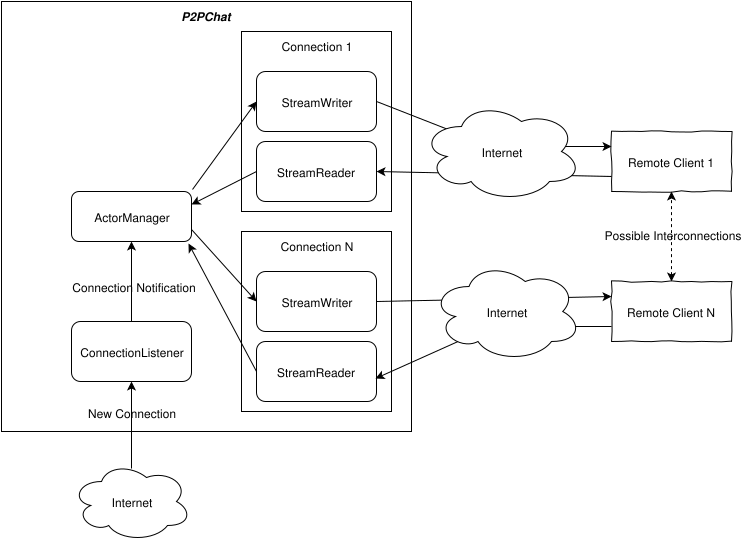
\includegraphics[width=\textwidth]{figures/p2pchat_structure.png}
  \caption{A small diagram showing a simplified overview of the different actors used in the chat system. Each arrow inside the \cmd{P2PChat} rectangle represents a channel between two actors. The actors use these channels in order to communicate and pass data to each other. Arraws across the border or outside of the rectangle represents a socket connection.}
  \label{fig:simple_overview}
\end{figure}

When the program is first executed it creates two new actors. One actor that listens for new tcp-connections called the \cmd{ConnectionListener} and one actor that keeps track of all connected clients and their associated actors. The tracking actor is called the \cmd{ActorManager}. The \cmd{ActorManager} is also the one responsible for propagating messages between all active connections. When it receives a new message it broadcasts it to all connection associated actors, which in turn send the message to their connected remote clients. A simplified overview of all actors and their intercommunication can be seen in figure \ref{fig:simple_overview}.

When a new connection is established the \cmd{ConnectionListener} will spawn two new actors. One listens for new data on the socket, and the other waits for data to send back over the socket. It then notifies the \cmd{ActorManager} about these two new actors and the connection they represent by sending it a message containing a new \cmd{Client} object.

The \cmd{ActorManager} receives the new \cmd{Client} object and stores it in its list of connected clients. When one of the clients sends a message to the program, the \cmd{StreamReader} will parse the message which is json-encoded and send the result to the \cmd{ActorManager}, which then passes it on to the rest of the connections.

\section{Performance Evaluation}
Since this implementation utilizes a peer-to-peer network, benchmarking becomes very complex and difficult. I was not unable to come up with a good benchmarking solution that could properly test the limitations of my system. I could have spun up $10,000$ clients that all attempted to connect to the same machine. But was unable to come up with a reliable enough solution that wasn't affected by my own machines resources in regards to opening lots of sockets and sending data.

Another solution would have been to create a single client that sends a lot of messages. But the remote client does not respond when receiving a regular message so I had nothing to work against from my local machine. I could have measured the resource usage at the remote machine, but since the program only creates a single receiver-actor per connection there would have been no parallelism to compare against when sending lots of messages from a single connection.

The third and possibly the best solution would have been to build up a large network of clients, and then trigger them to all spam a single client with lots of data and see how it fared to the pressure. Thus being able to see how well it scaled for large processing, depending on the resources available. But getting them all to send data at the exact same time, as well as setting it all up and collecting the measurements in a reliable manner would be an entirely different project.

\section{Concurrency Abstractions}
As described in section \ref{sec:documentation}, the abstraction model used in this project is the actor model \cite{agha1985actors}. It accomplishes this by using channels between all threads in the program. No locks are used anywhere, and no threads share any data with each other.

Using the actor model simplifies the parallelism. There are no locks to keep track of. And there's no data shared between threads that must be monitored.

However, since no shared data is allowed, it becomes tricky to establish some form of chat history since all actors can only modify their own private space. In the case of mutex-locks a common chat history can be established by having all threads share access to the same data structure, only appending messages to it when a new message has been received, and reading the log when needed.

In order to accomplish this with the current setup in regards to actors, each actor must maintain their own chat log. And because messages and data can be received in any order, this log has the probability of looking completely different depending on which actor you look at.

The mutex-lock based solution does not suffer this fragmentation issue since all threads read and write to the same log.

A similar solution in regards to the mutex-solution can be used with actors. Instead of having a shared data structure represent the chat log, an actor can be used instead. Any actor that wants to write to the log sends a message to the chat-actor; and any actor that wants to read the log sends another message to the chat-actor which then replies with the requested information.

\section{Known Shortcomings}
\subsection{Duplicate Messages}
If several clients are connected together in a network where some clients share neighbours, then it is possible for those clients to receive the same message several times. This is due to how clients broadcast messages naively to all of their network connections.

A solution to this could use some form of message identifier. If a clients receives a message with an id matching a previously received message it will simply ignore it. The problem with this solution is how to properly generate unique id's without conflicts. All clients need some form of synchronization between each other in order to avoid these conflicts.

It is possible that the id could be generated by performing a hashing of the entire message. Thus it should theoretically produce unique identifiers without the need of client synchronization.
